\section{Auswirkungen und Resultate von Zero-Trust}\label{sec:auswirkungen-und-resultate-von-zero-trust}

\subsection{Verbesserung der Sicherheitsebene}\label{subsec:verbesserung-der-sicherheitsebene}
Eine \ac{zta} trägt zur Verbesserung der Sicherheitsebene von Systemen bei, indem es einen Paradigmenwechsel in der Cybersicherheit darstellt.
Das Vertrauen in Personen, Geräte und Prozesse wird zuvor bereits dargestellt auf ein Minimum reduziert, wodurch die Sicherheit erhöht wird.

Zudem wird das Datenbewusstsein und die Dateneinsicht in einer \ac{zta} erhöht.
Hierdurch und durch die kontinuierliche Überwachung des Datenverkehrs ermöglicht es, sowohl verdächtige Verhaltensweisen und Angriffe schneller zu erkennen und zu unterbinden, als auch aus vergangenen Vorfällen Fehler zu erkennen und die bestehenden Sicherheitsmaßnahmen entsprechend anzupassen.\autocites[\vglf][\pagef 9]{cunningham-2019}[\vglf][\pagef 4]{buck-2021}
Durch Mikrosegmentierung, dem Aufteilen eines Netzwerkes in kleinere Segmente, und dem Gewähren von Zugriff ausschließlich auf die für die Anfrage benötigten Ressourcen wird sichergestellt, dass kein überflüssiger und ungewollter Datenverkehr durchgeführt wird.\autocite[\vglf][\pagef 30]{shore-2021}
Hierdurch wird die Anzahl der möglichen ausnutzbaren Lücken im System reduziert.

Ein nach \ac{zt} eingerichtetes Netzwerk ist außerdem weniger anfällig gegenüber Malware, da die segmentierten Bereiche des Netzwerkes es schwieriger bis unmöglich machen, die Malware im System zu verbreiten.
Allein das Betreten des Netzwerkes der Malware, nachdem \zb ein Mitarbeiter einen Phishing Link ausgeführt hat, wird erschwert, da die Daten durch die Netzwerkeinrichtung zunächst überprüft werden, bevor sie auf dem Gerät des Nutzers ankommen.\autocite[\vglf][\pagef 7]{cunningham-2019}
Bei Malware-Programmen werden entsprechende Trigger ausgelöst, die vor dem schädlichen Datenverkehr warnen.\autocite[\vglf][\pagef 7]{cunningham-2019}
Gleichzeitig kann eine \ac{zta} auch das Ausbreiten eines Malware-Programmes unterbinden, welches \zb über einen korrupten USB-Stick in das System eingebracht wird, da das Programm durch die Segmentierung nur schwierig auf andere Geräte im Netzwerk übergreifen kann.\autocite[\vglf][\pagef 7]{cunningham-2019}

\subsection{Reduzierung von Angriffsflächen}\label{subsec:reduzierung-von-angriffsflachen}
Durch die Mikrosegmentierung eines Netzwerks mit einer \ac{zta} in kleinere, isolierte Segmente werden Angriffe auf das Segment begrenzt, in dem sie stattfinden, ohne sich auf andere Segmente ausbreiten zu können.
Dies reduziert das Risiko von Datenlecks und unbefugtem Zugriff.\autocites[\vglf][\pagef 20]{shore-2021}[\vglf][\pagef 4]{buck-2021}
Besonders gegen \ac{ddos}-Angriffe bietet eine \ac{zta} starken Schutz, da die meist automatisierten Angriffe durch die Mikrosegmentierung nur geringe Bereiche des Systems anwählen können.\autocite[\vglf][\pagef 289]{Eidle-2017}

Des Weiteren trägt die Verwendung von \ac{sdp} dazu bei, dass eine Black Box gebildet wird, welche die Infrastruktur und Ressourcen vor öffentlichem Zugriff verbirgt.\autocites[\vglf][\pagef 4]{buck-2021}[\vglf][\pagef 1]{kumar-2019}

Die Möglichkeit, allen Datenverkehr zu überwachen trägt zudem dazu bei, den Schaden, den Datenausbrüche verursachen, zu begrenzen oder sogar ganz zu verhindern.\autocite[\vglf][\pagef 6]{cunningham-2019}
Viele Lösungen benötigen Wochen bis Monate, um einen Vorfall zu erkennen, sodass in vielen Fällen externe Akteure wie Kunden oder Partner die Firma über den Vorfall informieren.\autocite[\vglf][\pagef 6]{cunningham-2019}
Mit bisher genutzten Lösungen beträgt die Zeit, die es benötigt wird, über einen Sicherheitsvorfall benachrichtigt zu werden, im Median $78$ Tage.\autocite[\vglf][\pagef 5]{fireeye-2019}

Die Segmentierung eines Netzwerkes trägt außerdem dazu, der Schnelllebigkeit der Technologien und Netzwerke, sowie den Problemen beim Bearbeiten und Schützen der Schwachstellen entgegenzuwirken.
So wurden zum Beispiel im Jahr $2018$ allein wurden ungefähr $16.500$ Einträge der \ac{nvd} der USA hinzugefügt, im Jahr $2022$ bereits ungefähr $25.200$ \autocites[\vglf][\pagef 6]{cunningham-2019}[\vglf][]{cve-2023}.

\subsection{Schutz sensibler Daten}\label{subsec:schutz-sensibler-daten}
\todo[inline]{Eventuell subsection \enquote{Datenverarbeitung} nennen und zwei subsubsections zu \enquote{Datenschutz} und \enquote{Datenspeicherung} schreiben?}
Um eine \ac{zta} einzurichten werden im Allgemeinen fünf Schritte vorausgesetzt.
Diese sind (\lowerromannumeral{1}) das Identifizieren der sensiblen Daten, (\lowerromannumeral{2}) das Erfassen des Datenflusses der sensiblen Daten, (\lowerromannumeral{3}) der Entwurf der \ac{zt}-Parametern, (\lowerromannumeral{4}) das kontinuierliche Überwachen des Systems mit Sicherheitsanalysen und (\lowerromannumeral{5}) das Einführen der Steuerung und Automatisierung der Sicherheitsmaßnahmen.\autocites[\vglf][\pagef 2-3]{ahmed-2020}[\vglf][]{balaouras-2023}

Zusätzlich werden in einer \ac{zta} viele Daten, darunter auch Nutzerdaten gespeichert, damit sichergestellt werden kann, welcher Akteur auf welche Daten, Systeme und Dienste zugreifen kann, \bzw darf.
Für diese Daten wird für jeden Akteur ein Register eingerichtet, welches die folgenden Daten beinhalten kann\autocite[\vglf][\pagef 161]{colombo-2021}:
\begin{itemize}
    \item die Anzahl der erfolgreichen und nicht erfolgreichen Verbindungsanfragen, sowie die Frequenz dieser;
    \item jeder in Anspruch genommene Dienst, der zu einer Zugriffsentscheidung führt, und für jeden dieser Dienste die Häufigkeit und Anzahl dieser Anfragen;
    \item jede angeforderte Datenressource, die dem Subjet erlaubt und verweigert wurde, zusammen mit dem zugehörigen Ressourcentyp\footnote{\zb Datensatz, Zeilendaten, Datenstrom} und der Empfindlichkeitsstufe, der Zugriffsart\footnote{\zb Lesen, Schreiben, Lesen und Schreiben} und die Dauer\footnote{\zb sofort/kontinuierlich und die zugehörige Länge} sowie alle verfügbaren Daten, die den Zugriffskontext bezeichnen, wie \zb Zeit, Ort und Systemzustand;
    \item die Historie aller dem Akteur entzogenen Berechtigungen;
    \item aktueller Satz von Akteursattributen zusammen mit jeder beobachteten Änderung dieser Eigenschaften.
\end{itemize}

\subsection{Probleme}\label{subsec:probleme}
\autoref{fig:zero-trust-challenges} zeigt, welchen Problemen Unternehmen weltweit begegnen, die sie daran hindern, eine \ac{zta} in ihrem Unternehmen einzurichten.\autocite[\vglf][]{fortinet-2023}
\begin{figure}[htbp]
    \centering
    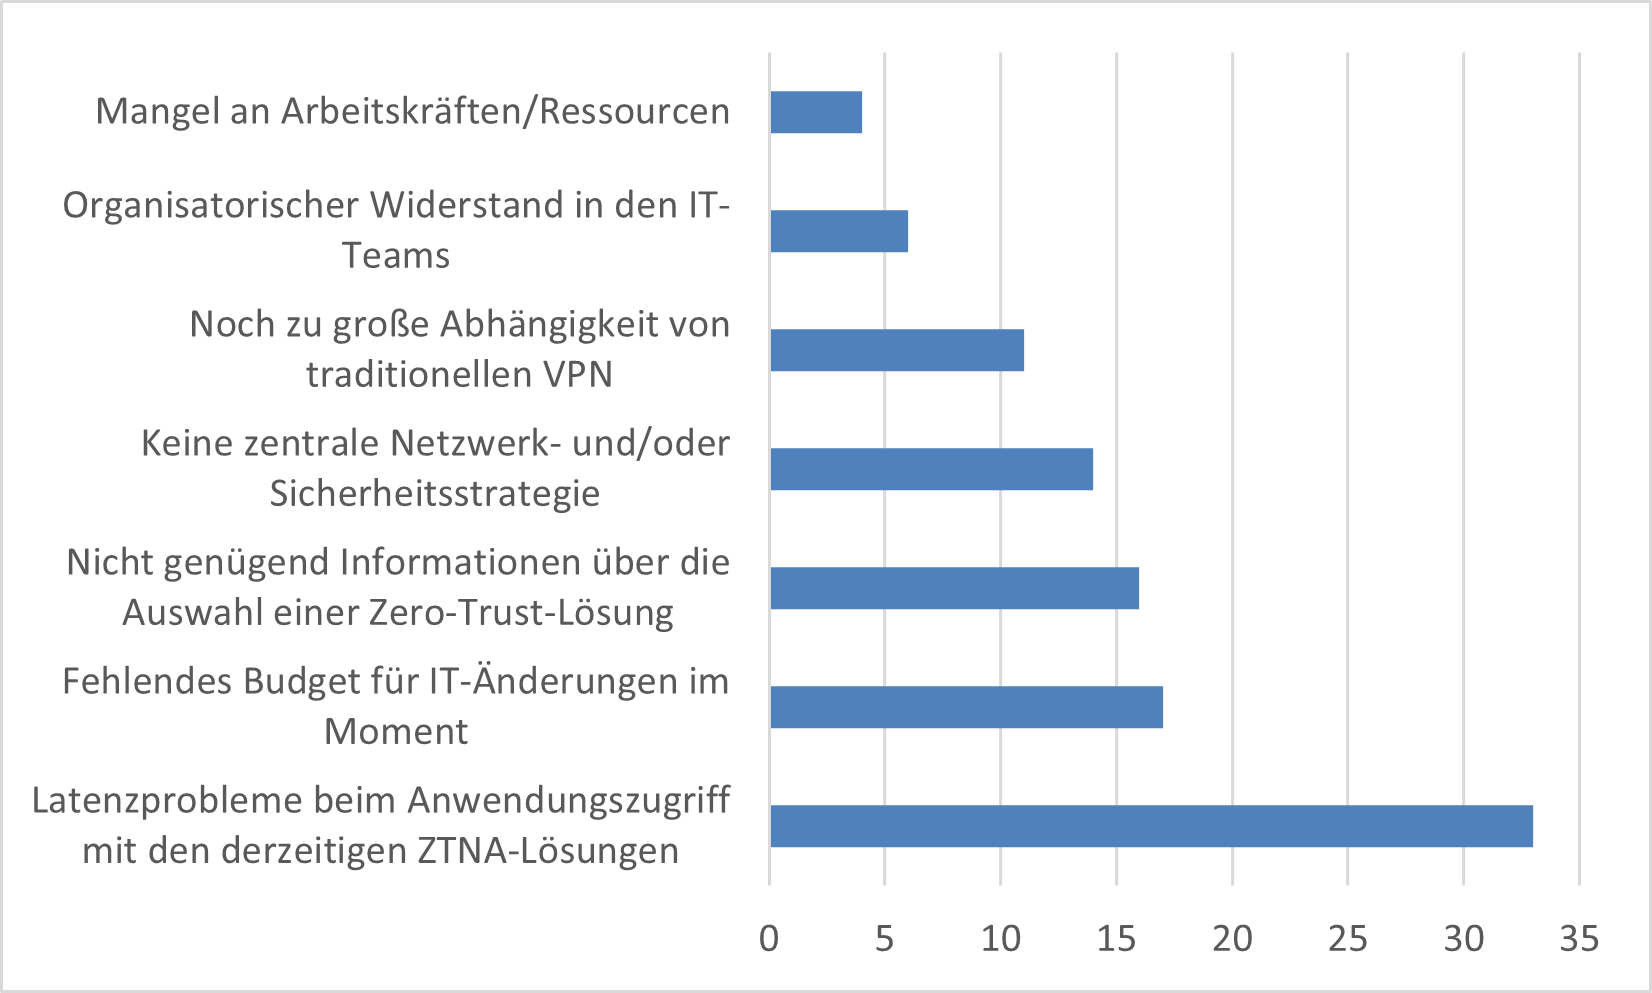
\includegraphics[width=0.75\textwidth, trim = {0.2cm 0.3cm 0.4cm 0.25cm}, clip]{src/abbildungen/Herausforderungen_ZeroTrust}
    \captionsetup{width=\linewidth, format=hang}
    \caption[Wichtigste Herausforderungen beim Aufbau einer weltweiten Zero-Trust-Strategie im Jahr 2023]{Wichtigste Herausforderungen beim Aufbau einer weltweiten Zero-Trust-Strategie im Jahr 2023\newline Werte in Prozent}
    \label{fig:zero-trust-challenges}
\end{figure}

Zusätzlich zu diesen Problemen gibt es beim Aufbau einer \ac{zta} auch die Bedenken um die Sicherheit gespeicherter Daten, welche wie in \autoref{subsec:schutz-sensibler-daten} aufgeführt wurden zur effektiven Zugriffsüberprüfung erforderlich sind.
Jedoch ist es möglich, auch diese Daten innerhalb der \ac{zta} zu speichern, sodass auch sie von dem Schutz des Netzwerkes profitieren.
Hierbei muss allerdings beachtet werden, dass die Systeme und Akteure, die Einfluss auf die Zugriffsentscheidung über Anfragen von Systemen und Nutzern haben, auch auf die gespeicherten Daten Zugriff besitzen müssen, andernfalls bringt die Speicherung der Daten keinen nutzen.

Darüber hinaus kann es für Unternehmen zu Problemen kommen, wenn eine \ac{zta} eingerichtet werden soll, da die betroffenen Systeme während der Einführung nicht nutzbar sind.
Da eine \ac{zta} aber in bestehende Systeme partiell eingeführt werden kann, ist dies nur ein kleines Hindernis.


